\chapter{APPENDIX A: DSAM CURVES}
\section{$^{160}$Gd at E$_n$=1.5~MeV}\label{app:DSAM_Gd_15}
The next 3 pages contain the Doppler Shift plots for the Gadolinium campaign at a neutron energy of 1.5~MeV.
\newpage
\begin{center}
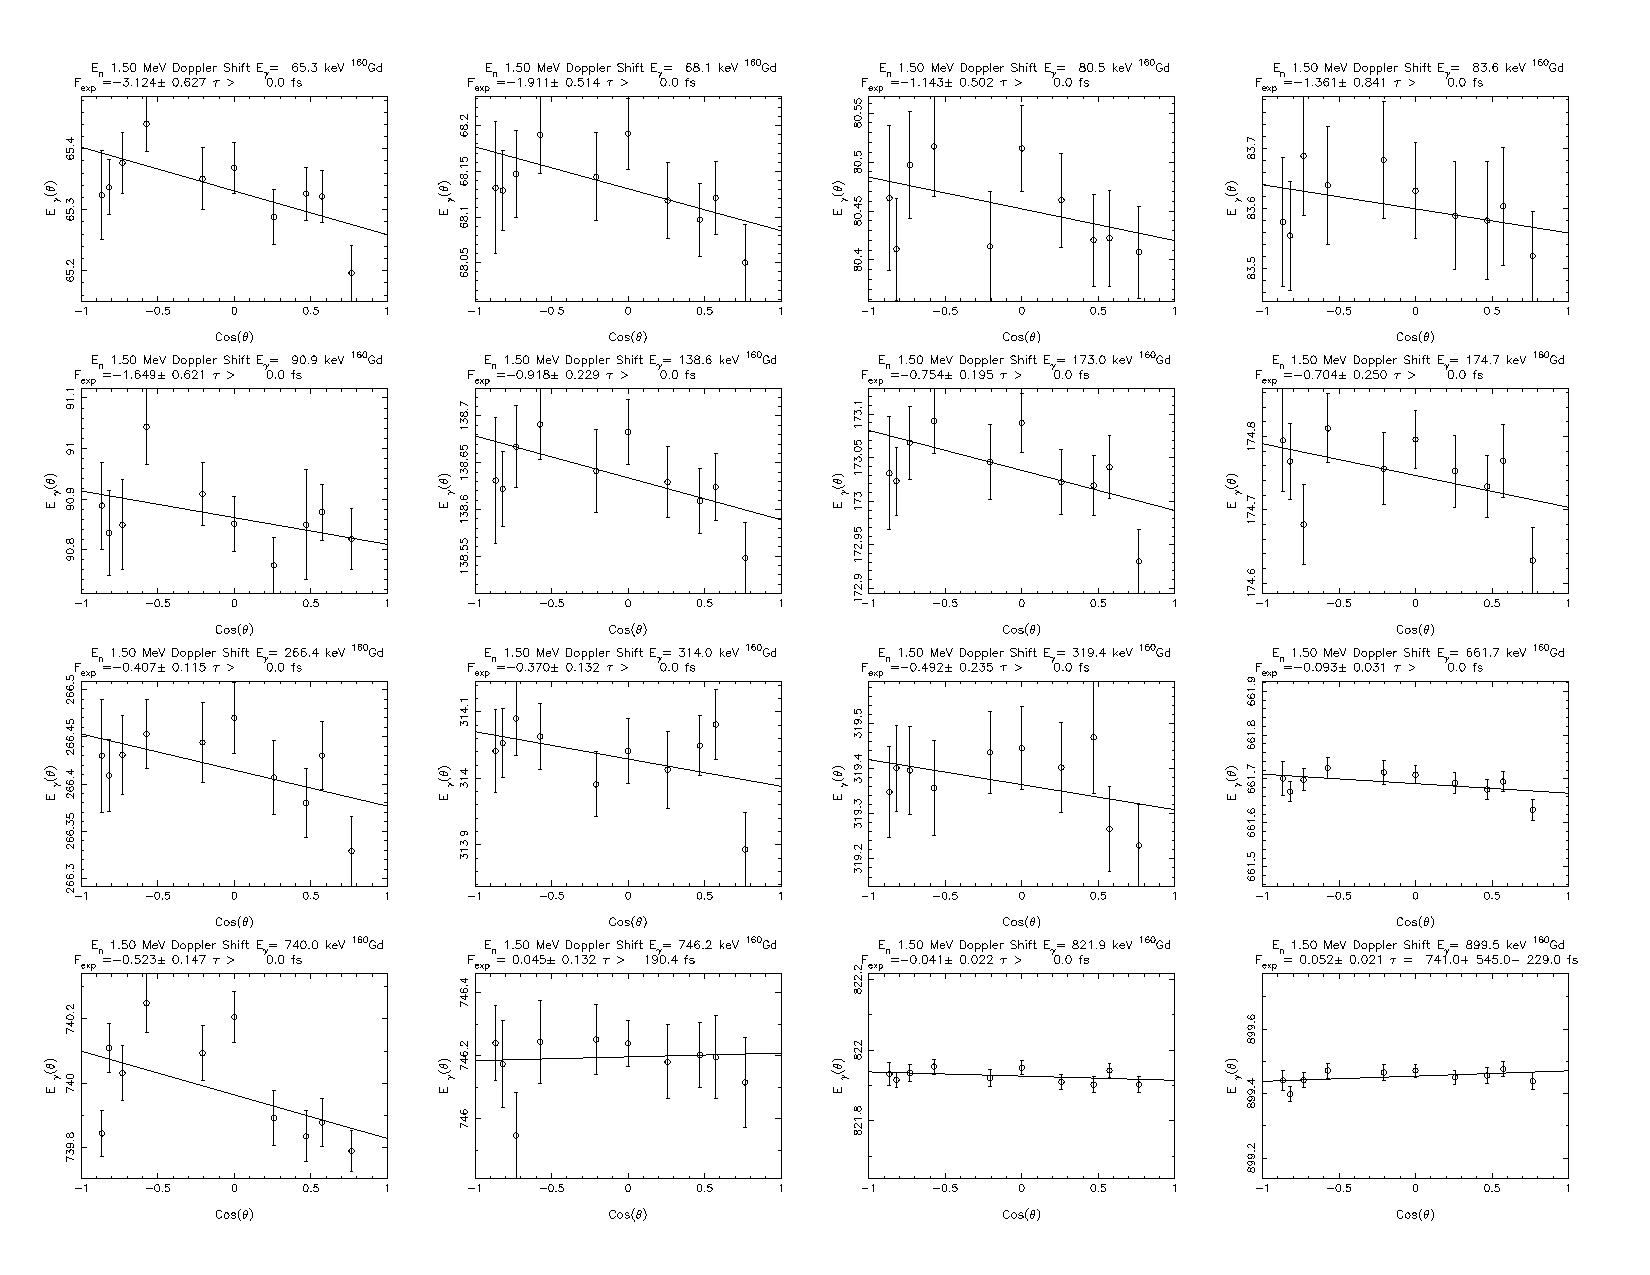
\includegraphics[page=1,angle=90,height=0.95\textheight]{160Gd_15_DSAM.pdf}
\end{center}
\begin{center}
\includegraphics[page=2,angle=90,height=0.95\textheight]{160Gd_15_DSAM.pdf}
\end{center}
\begin{center}
\includegraphics[page=3,angle=90,height=0.95\textheight]{160Gd_15_DSAM.pdf}
\end{center}
\section{$^{160}$Gd at E$_n$=2.0~MeV}\label{app:DSAM_Gd_20}
The bulk of the extracted lifetimes from the $^{160}$Gd experiments stem from the 2.0~MeV dataset. Listed below are the DSAM-plots for this bombarding neutron energy.
\begin{center}
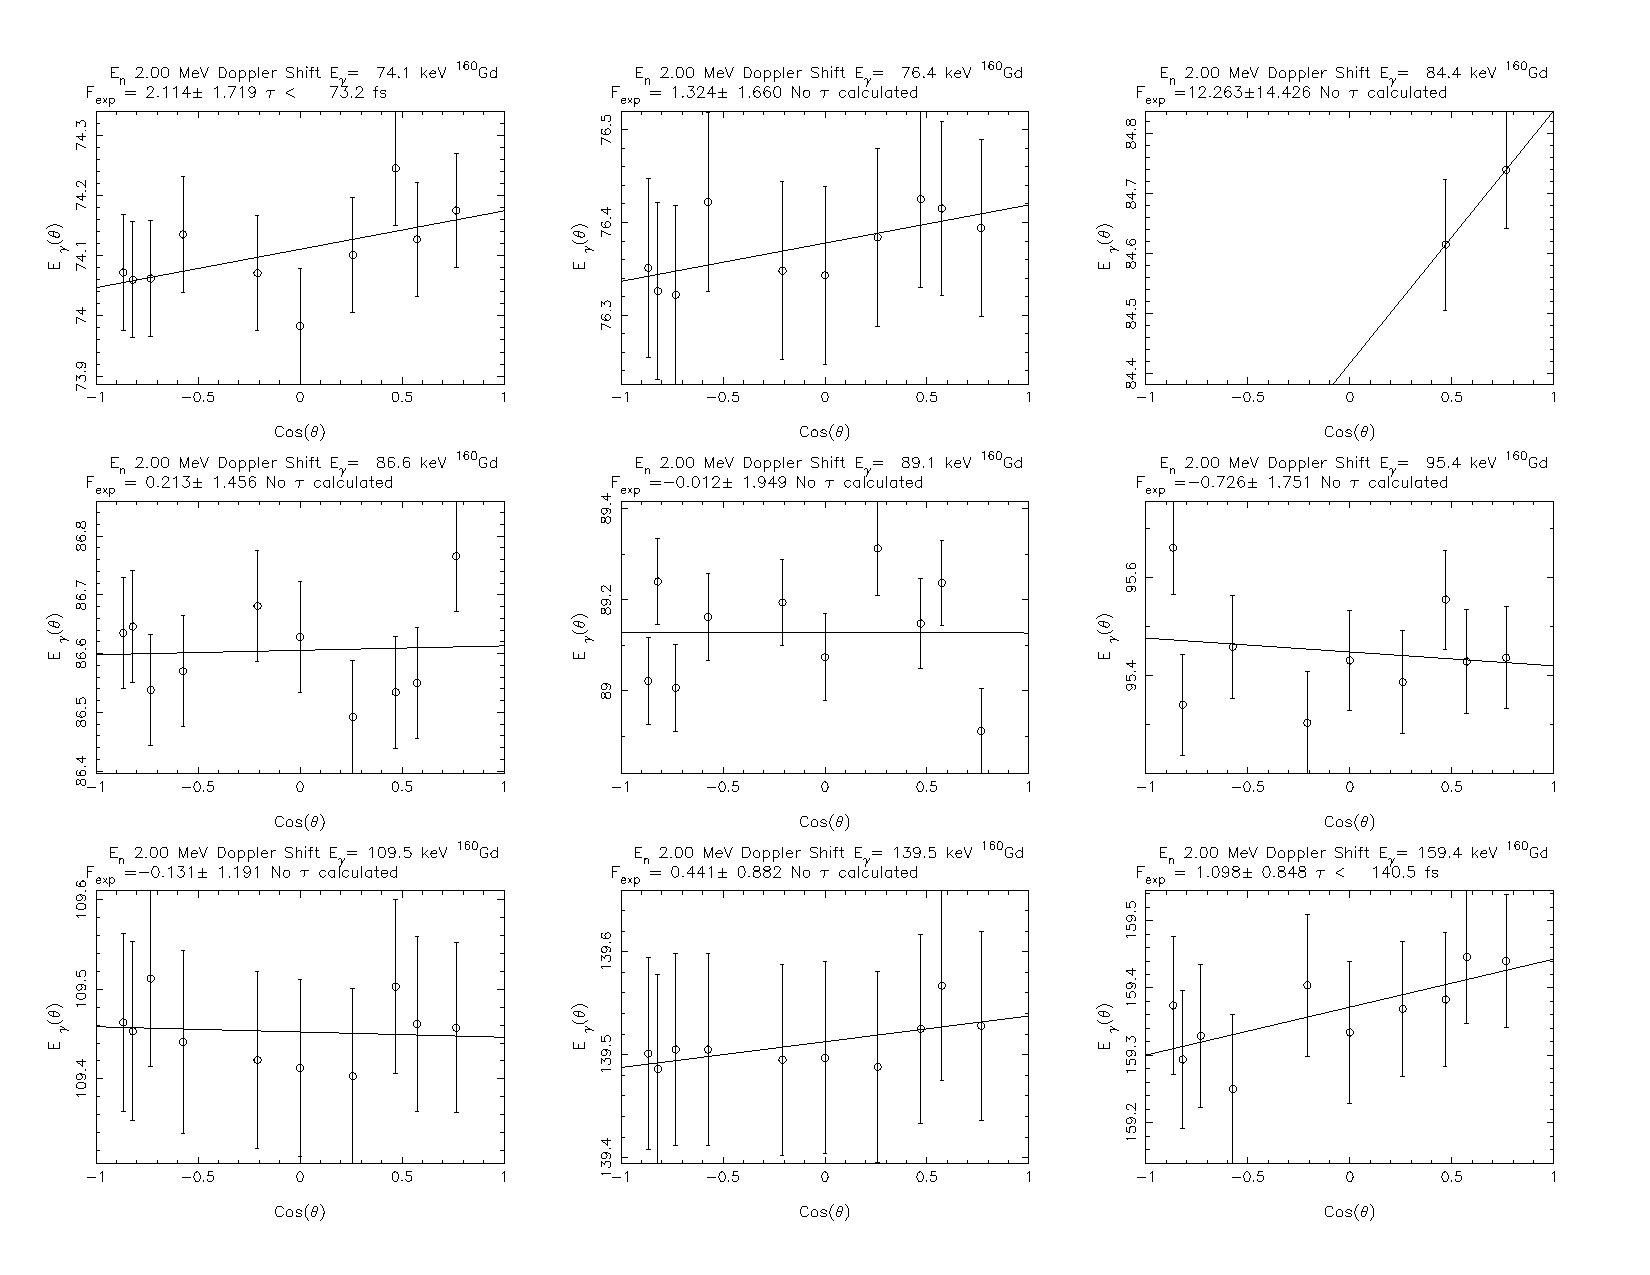
\includegraphics[page=1,angle=90,height=0.95\textheight]{160Gd_20_DSAM.pdf}
\end{center}
\begin{center}
\includegraphics[page=2,angle=90,height=0.95\textheight]{160Gd_20_DSAM.pdf}
\end{center}
\begin{center}
\includegraphics[page=3,angle=90,height=0.95\textheight]{160Gd_20_DSAM.pdf}
\end{center}
\begin{center}
\includegraphics[page=4,angle=90,height=0.95\textheight]{160Gd_20_DSAM.pdf}
\end{center}
\begin{center}
\includegraphics[page=5,angle=90,height=0.95\textheight]{160Gd_20_DSAM.pdf}
\end{center}
\begin{center}
\includegraphics[page=6,angle=90,height=0.95\textheight]{160Gd_20_DSAM.pdf}
\end{center}
\begin{center}
\includegraphics[page=7,angle=90,height=0.95\textheight]{160Gd_20_DSAM.pdf}
\end{center}
\begin{center}
\includegraphics[page=8,angle=90,height=0.95\textheight]{160Gd_20_DSAM.pdf}
\end{center}
\begin{center}
\includegraphics[page=9,angle=90,height=0.95\textheight]{160Gd_20_DSAM.pdf}
\end{center}
\begin{center}
\includegraphics[page=10,angle=90,height=0.95\textheight]{160Gd_20_DSAM.pdf}
\end{center}
\begin{center}
\includegraphics[page=11,angle=90,height=0.95\textheight]{160Gd_20_DSAM.pdf}
\end{center}
\begin{center}
\includegraphics[page=12,angle=90,height=0.95\textheight]{160Gd_20_DSAM.pdf}
\end{center}
\begin{center}
\includegraphics[page=13,angle=90,height=0.95\textheight]{160Gd_20_DSAM.pdf}
\end{center}
\begin{center}
\includegraphics[page=14,angle=90,height=0.95\textheight]{160Gd_20_DSAM.pdf}
\end{center}
\begin{center}
\includegraphics[page=15,angle=90,height=0.95\textheight]{160Gd_20_DSAM.pdf}
\end{center}
\begin{center}
\includegraphics[page=16,angle=90,height=0.95\textheight]{160Gd_20_DSAM.pdf}
\end{center}

\section{$^{160}$Gd at E$_n$=2.8~MeV}\label{app:DSAM_Gd_28}%LE until pg 24, HE 24-25
Long-lived calibrants for the 2.8~MeV neutron (n,n$^\prime\gamma$) experiment on $^{160}$Gd include the ground state 4$^+\rightarrow$2$^+$ transition (173~keV), the $^1$H(n,d) reaction at 2.223~MeV, and the $^{23}$Na line at 2754~keV.
\begin{center}
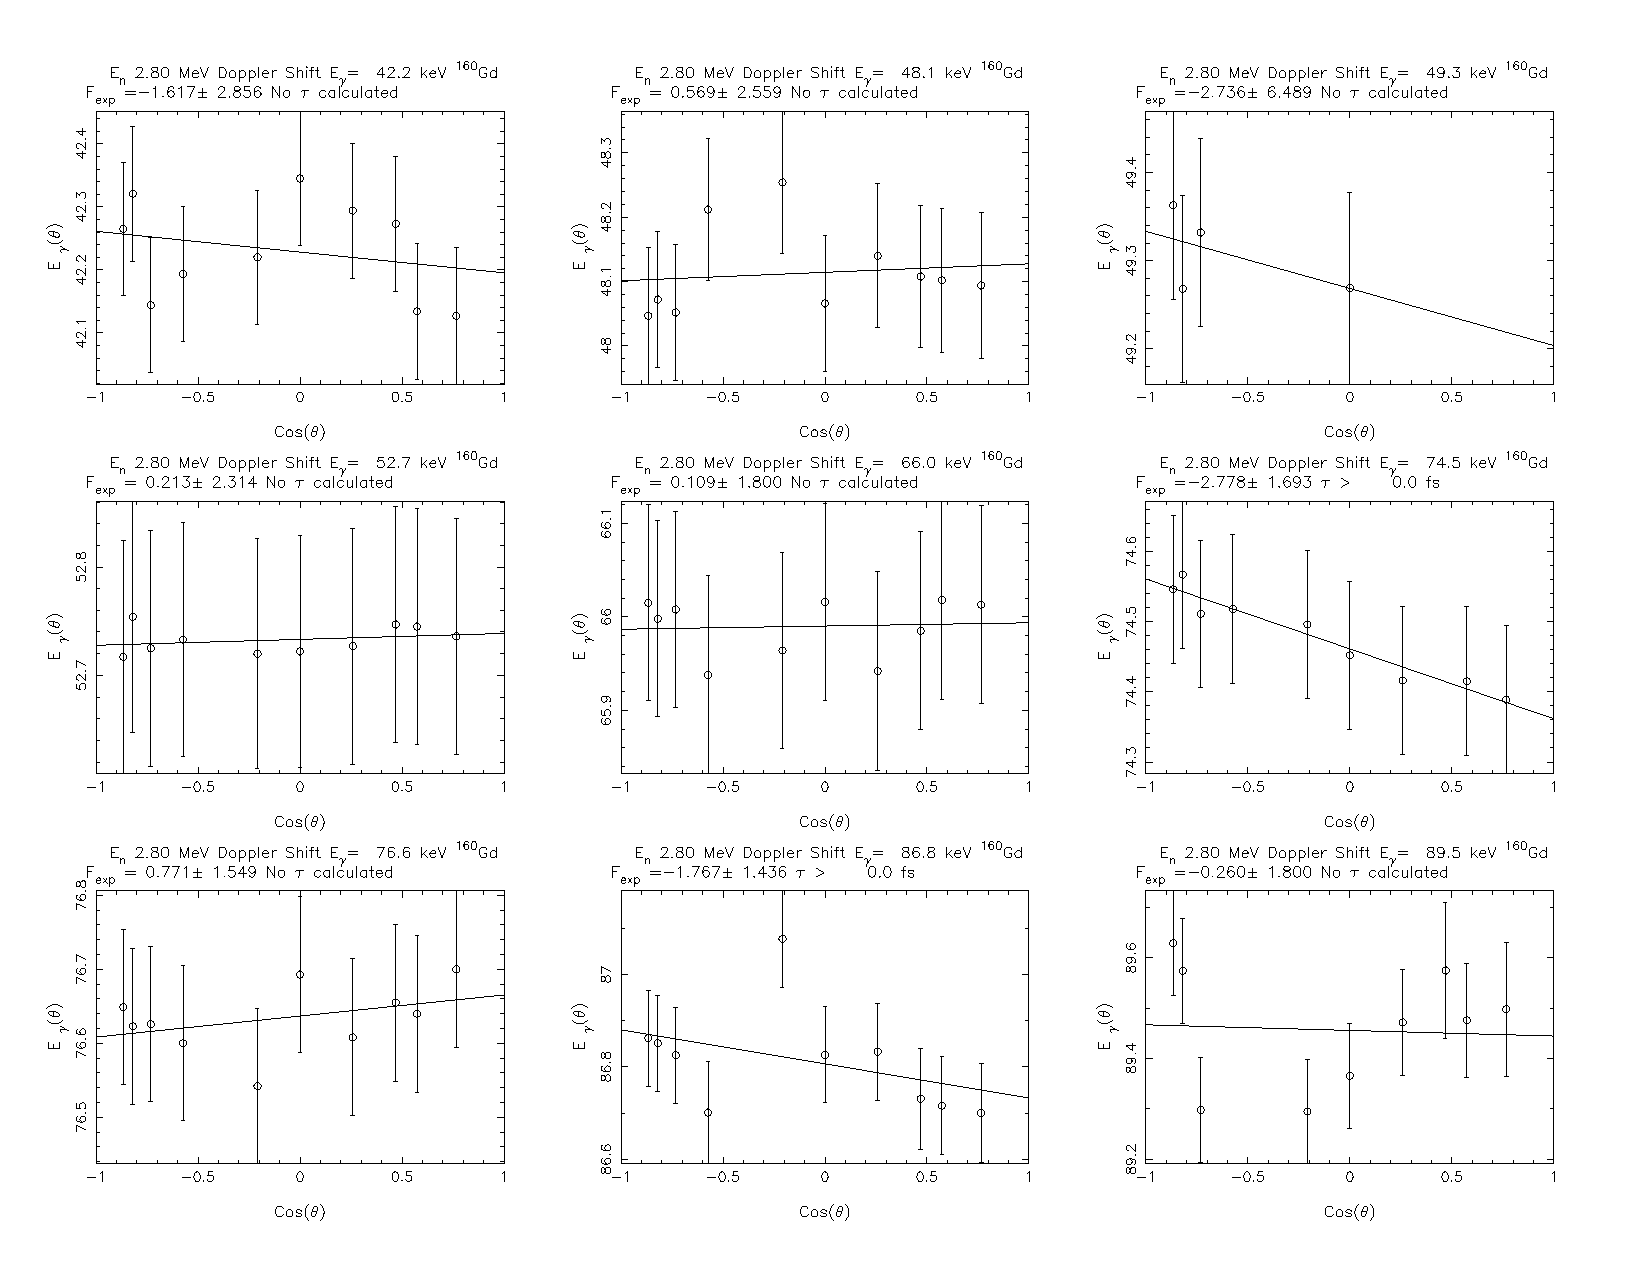
\includegraphics[page=1,angle=90,height=0.95\textheight]{160Gd_28ftau_LE_no.pdf}
\end{center}
\begin{center}
\includegraphics[page=2,angle=90,height=0.95\textheight]{160Gd_28ftau_LE_no.pdf}
\end{center}
\begin{center}
\includegraphics[page=3,angle=90,height=0.95\textheight]{160Gd_28ftau_LE_no.pdf}
\end{center}
\begin{center}
\includegraphics[page=4,angle=90,height=0.95\textheight]{160Gd_28ftau_LE_no.pdf}
\end{center}
\begin{center}
\includegraphics[page=5,angle=90,height=0.95\textheight]{160Gd_28ftau_LE_no.pdf}
\end{center}
\begin{center}
\includegraphics[page=6,angle=90,height=0.95\textheight]{160Gd_28ftau_LE_no.pdf}
\end{center}
\begin{center}
\includegraphics[page=7,angle=90,height=0.95\textheight]{160Gd_28ftau_LE_no.pdf}
\end{center}
\begin{center}
\includegraphics[page=8,angle=90,height=0.95\textheight]{160Gd_28ftau_LE_no.pdf}
\end{center}
\begin{center}
\includegraphics[page=9,angle=90,height=0.95\textheight]{160Gd_28ftau_LE_no.pdf}
\end{center}
\begin{center}
\includegraphics[page=10,angle=90,height=0.95\textheight]{160Gd_28ftau_LE_no.pdf}
\end{center}
\begin{center}
\includegraphics[page=11,angle=90,height=0.95\textheight]{160Gd_28ftau_LE_no.pdf}
\end{center}
\begin{center}
\includegraphics[page=12,angle=90,height=0.95\textheight]{160Gd_28ftau_LE_no.pdf}
\end{center}
\begin{center}
\includegraphics[page=13,angle=90,height=0.95\textheight]{160Gd_28ftau_LE_no.pdf}
\end{center}
\begin{center}
\includegraphics[page=14,angle=90,height=0.95\textheight]{160Gd_28ftau_LE_no.pdf}
\end{center}
\begin{center}
\includegraphics[page=15,angle=90,height=0.95\textheight]{160Gd_28ftau_LE_no.pdf}
\end{center}
\begin{center}
\includegraphics[page=16,angle=90,height=0.95\textheight]{160Gd_28ftau_LE_no.pdf}
\end{center}
\begin{center}
\includegraphics[page=17,angle=90,height=0.95\textheight]{160Gd_28ftau_LE_no.pdf}
\end{center}
\begin{center}
\includegraphics[page=18,angle=90,height=0.95\textheight]{160Gd_28ftau_LE_no.pdf}
\end{center}
\begin{center}
\includegraphics[page=19,angle=90,height=0.95\textheight]{160Gd_28ftau_LE_no.pdf}
\end{center}
\begin{center}
\includegraphics[page=20,angle=90,height=0.95\textheight]{160Gd_28ftau_LE_no.pdf}
\end{center}
\begin{center}
\includegraphics[page=21,angle=90,height=0.95\textheight]{160Gd_28ftau_LE_no.pdf}
\end{center}
\begin{center}
\includegraphics[page=22,angle=90,height=0.95\textheight]{160Gd_28ftau_LE_no.pdf}
\end{center}
\begin{center}
\includegraphics[page=23,angle=90,height=0.95\textheight]{160Gd_28ftau_LE_no.pdf}
\end{center}
\begin{center}
\includegraphics[page=24,angle=90,height=0.95\textheight]{160Gd_28ftau_HE_no.pdf}
\end{center}
\begin{center}
\includegraphics[page=25,angle=90,height=0.95\textheight]{160Gd_28ftau_HE_no.pdf}
\end{center}
\section{$^{162}$Dy at E$_n$=1.6~MeV}\label{app:DSAM_Dy_16}
Listed below are the DSAM plots for the E$_n$=1.6~MeV dataset in $^{162}$Dy. Shown are the long-lived calibrants at 185~keV and 2223.3~keV (4$^+\rightarrow$2$^+$ and $^1$H(n,d), respectively).
\begin{center}
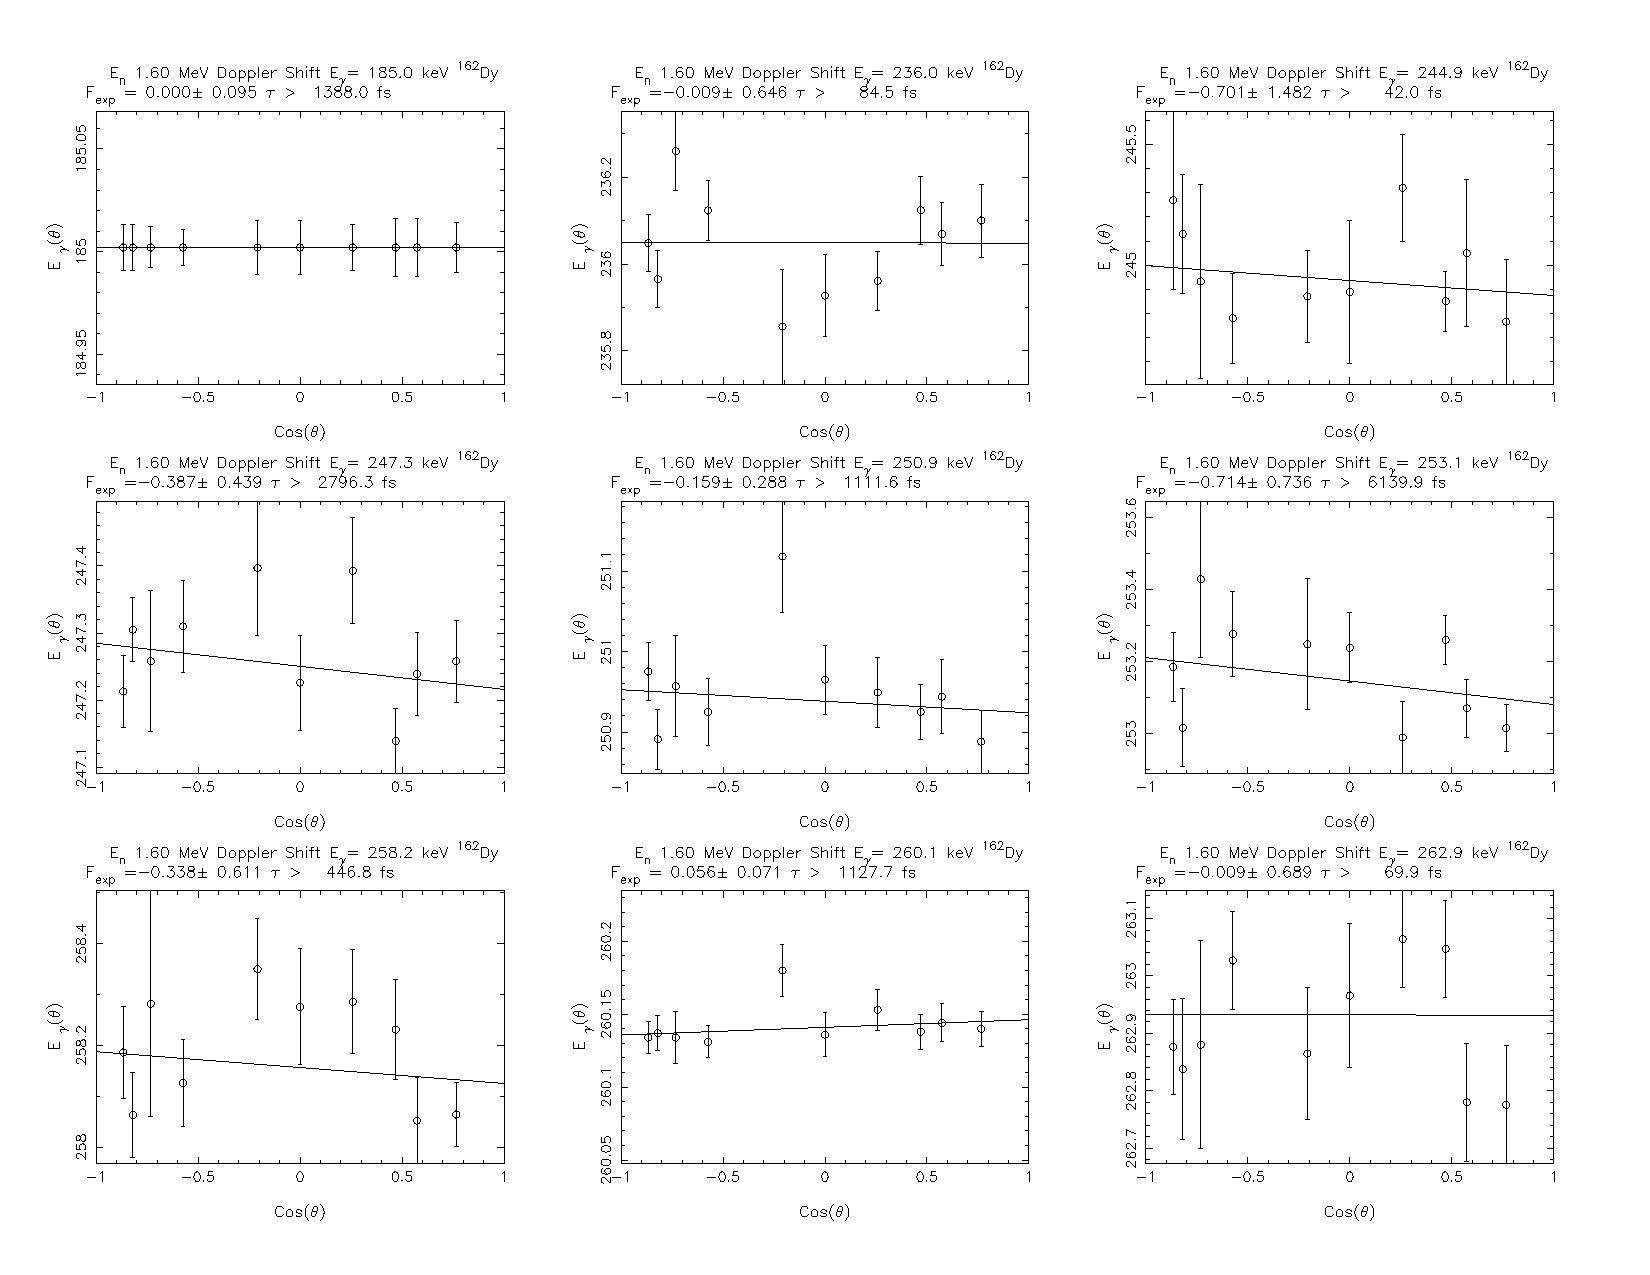
\includegraphics[page=1,angle=90,height=0.95\textheight]{162Dy_ftau_160_n.pdf}
\end{center}

\begin{center}
\includegraphics[page=2,angle=90,height=0.95\textheight]{162Dy_ftau_160_n.pdf}
\end{center}

\begin{center}
\includegraphics[page=3,angle=90,height=0.95\textheight]{162Dy_ftau_160_n.pdf}
\end{center}

\begin{center}
\includegraphics[page=4,angle=90,height=0.95\textheight]{162Dy_ftau_160_n.pdf}
\end{center}

\begin{center}
\includegraphics[page=5,angle=90,height=0.95\textheight]{162Dy_ftau_160_n.pdf}
\end{center}
\section{$^{162}$Dy at E$_n$=2.2~MeV}\label{app:DSAM_Dy_22}
Listed below are the DSAM plots for the E$_n$=2.2~MeV dataset for $^{162}$Dy.

Of note:

\begin{itemize}
\item Energies are piece-wise linearly calibrated to known, long-lived isomers or calibrant decays.
\item For example, E$_\gamma<$1332.4~keV are `clamped' at the ground state 4$^+\rightarrow$2$^+$ transition, the 185~keV $\gamma$ ray, and to the $^{60}$Co line at 1332.2~keV.
\item Any $\gamma$ ray above 1332.4~keV is calibrated to the 1173~keV $^{60}$Co line and the $^1$H(n,d) line at 2223.3~keV. (Any $\gamma$ decays in the overlap region are taken from the `LE' files - $<$1332~keV)
\end{itemize}

\begin{center}
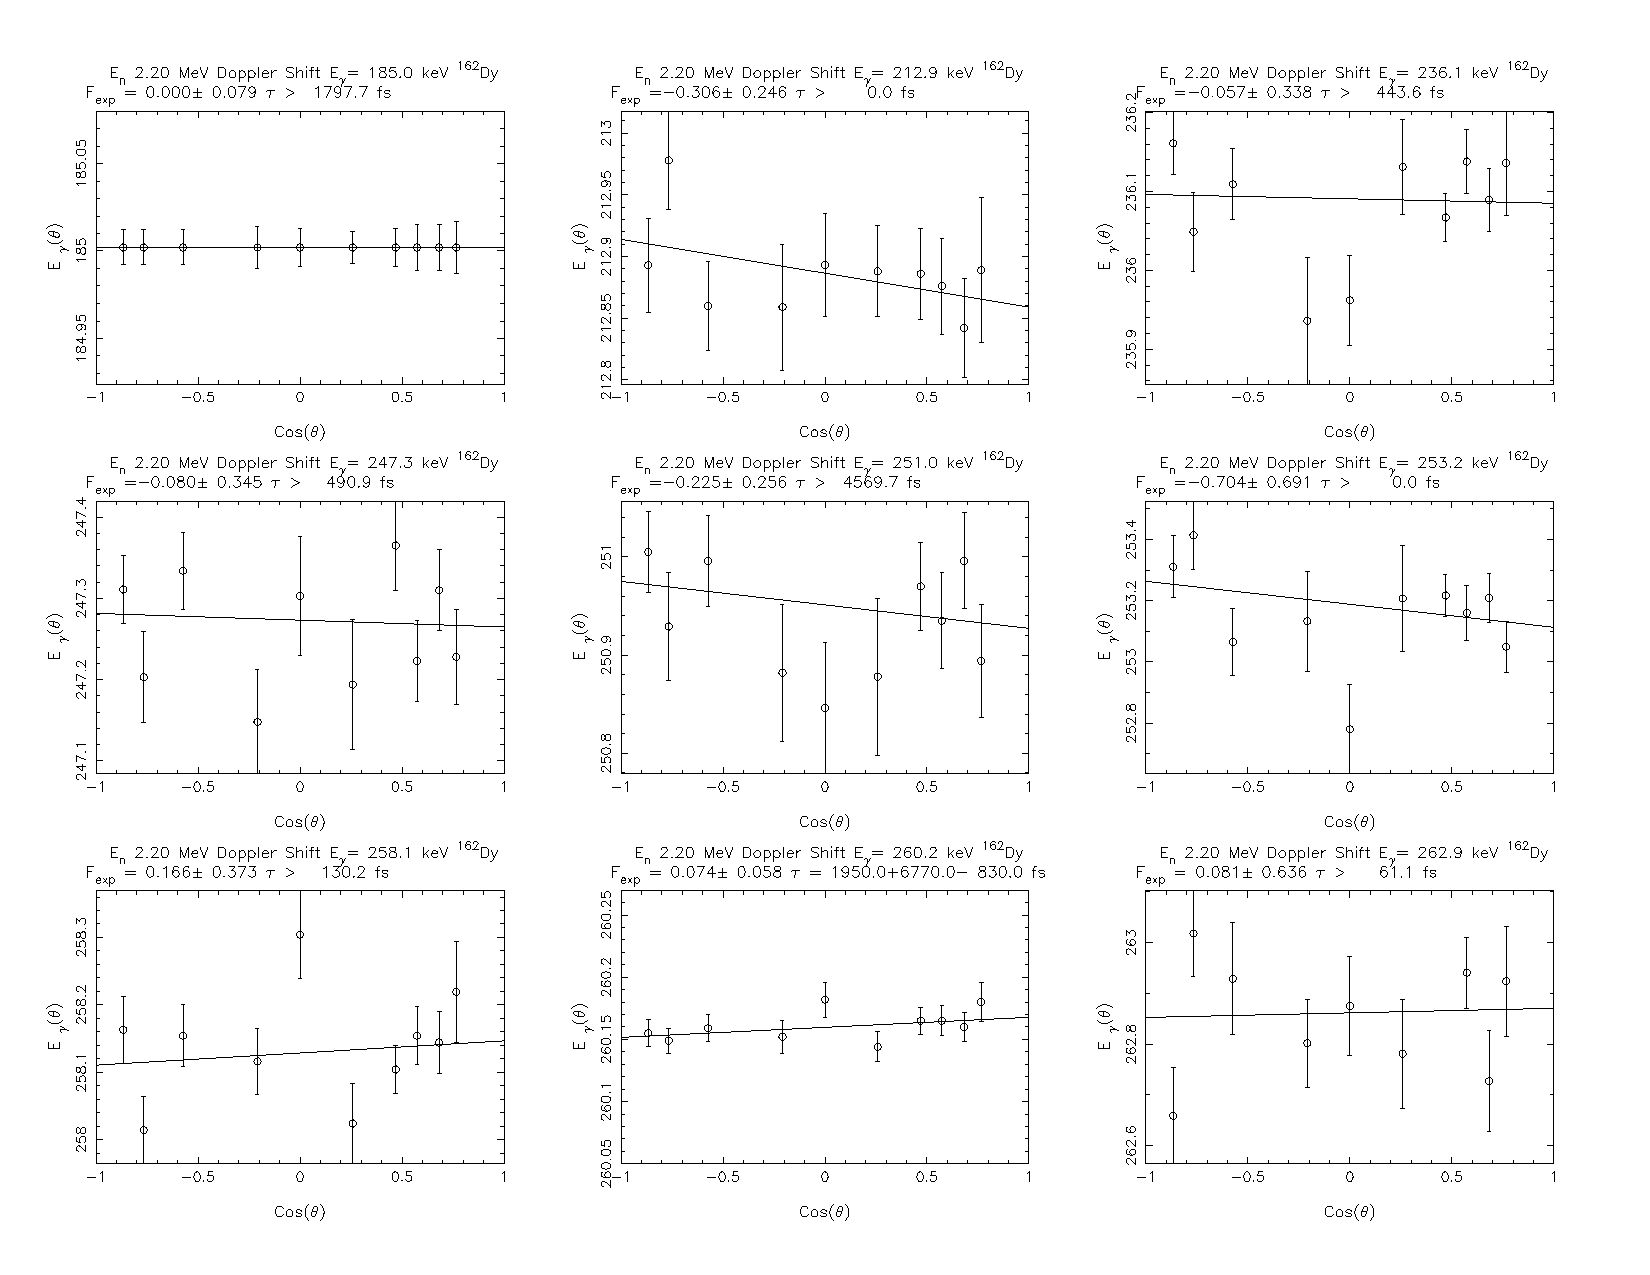
\includegraphics[page=1,angle=90,height=0.95\textheight]{162Dy_ftau_220_LE_n.pdf}
\end{center}
\begin{center}
\includegraphics[page=2,angle=90,height=0.95\textheight]{162Dy_ftau_220_LE_n.pdf}
\end{center}
\begin{center}
\includegraphics[page=3,angle=90,height=0.95\textheight]{162Dy_ftau_220_LE_n.pdf}
\end{center}
\begin{center}
\includegraphics[page=4,angle=90,height=0.95\textheight]{162Dy_ftau_220_LE_n.pdf}
\end{center}
\begin{center}
\includegraphics[page=5,angle=90,height=0.95\textheight]{162Dy_ftau_220_LE_n.pdf}
\end{center}
\begin{center}
\includegraphics[page=6,angle=90,height=0.95\textheight]{162Dy_ftau_220_LE_n.pdf}
\end{center}
\begin{center}
\includegraphics[page=7,angle=90,height=0.95\textheight]{162Dy_ftau_220_LE_n.pdf}
\end{center}
\begin{center}
\includegraphics[page=8,angle=90,height=0.95\textheight]{162Dy_ftau_220_LE_n.pdf}
\end{center}
\begin{center}
\includegraphics[page=9,angle=90,height=0.95\textheight]{162Dy_ftau_220_LE_n.pdf}
\end{center}
\begin{center}
\includegraphics[page=10,angle=90,height=0.95\textheight]{162Dy_ftau_220_LE_n.pdf}
\end{center}
\begin{center}
\includegraphics[page=11,angle=90,height=0.95\textheight]{162Dy_ftau_220_LE_n.pdf}
\end{center}
\begin{center}
\includegraphics[page=12,angle=90,height=0.95\textheight]{162Dy_ftau_220_HE_n.pdf}
\end{center}
\begin{center}
\includegraphics[page=13,angle=90,height=0.95\textheight]{162Dy_ftau_220_HE_n.pdf}
\end{center}
\begin{center}
\includegraphics[page=14,angle=90,height=0.95\textheight]{162Dy_ftau_220_HE_n.pdf}
\end{center}
\begin{center}
\includegraphics[page=15,angle=90,height=0.95\textheight]{162Dy_ftau_220_HE_n.pdf}
\end{center}


\section{$^{162}$Dy at E$_n$=3.1~MeV}\label{app:DSAM_Dy_31}
Listed below are the DSAM plots for the E$_n$=3.1~MeV dataset in $^{162}$Dy.

Similar to the $^{162}$Dy at E$_n$=2.2~MeV, there are regions of piece-wise linearity in the extraction of lifetimes.

\begin{itemize}
\item 185$<$E$_\gamma<$1332.2~keV (4$^+\rightarrow$2$^+$ \& $^{60}$Co)
\item 1332.2$<$E$_\gamma<$2223.3~keV ($^{60}$Co \& $^1$H(n,d))
\item 2223.3$<$E$_\gamma<$2754.6~keV ($^1$H(n,d) \& $^{23}$Na)
\end{itemize}
\newpage
\begin{center}
\includegraphics[page=1,angle=90,height=0.95\textheight]{162Dy_ftau_310_LE_n.pdf}
\end{center}
\begin{center}
\includegraphics[page=2,angle=90,height=0.95\textheight]{162Dy_ftau_310_LE_n.pdf}
\end{center}
\begin{center}
\includegraphics[page=3,angle=90,height=0.95\textheight]{162Dy_ftau_310_LE_n.pdf}
\end{center}
\begin{center}
\includegraphics[page=4,angle=90,height=0.95\textheight]{162Dy_ftau_310_LE_n.pdf}
\end{center}
\begin{center}
\includegraphics[page=5,angle=90,height=0.95\textheight]{162Dy_ftau_310_LE_n.pdf}
\end{center}
\begin{center}
\includegraphics[page=6,angle=90,height=0.95\textheight]{162Dy_ftau_310_LE_n.pdf}
\end{center}
\begin{center}
\includegraphics[page=7,angle=90,height=0.95\textheight]{162Dy_ftau_310_LE_n.pdf}
\end{center}
\begin{center}
\includegraphics[page=8,angle=90,height=0.95\textheight]{162Dy_ftau_310_LE_n.pdf}
\end{center}
\begin{center}
\includegraphics[page=9,angle=90,height=0.95\textheight]{162Dy_ftau_310_LE_n.pdf}
\end{center}
\begin{center}
\includegraphics[page=10,angle=90,height=0.95\textheight]{162Dy_ftau_310_LE_n.pdf}
\end{center}
\begin{center}
\includegraphics[page=11,angle=90,height=0.95\textheight]{162Dy_ftau_310_LE_n.pdf}
\end{center}
\begin{center}
\includegraphics[page=12,angle=90,height=0.95\textheight]{162Dy_ftau_310_LE_n.pdf}
\end{center}
\begin{center}
\includegraphics[page=13,angle=90,height=0.95\textheight]{162Dy_ftau_310_LE_n.pdf}
\end{center}
\begin{center}
\includegraphics[page=14,angle=90,height=0.95\textheight]{162Dy_ftau_310_LE_n.pdf}
\end{center}
\begin{center}
\includegraphics[page=15,angle=90,height=0.95\textheight]{162Dy_ftau_310_LE_n.pdf}
\end{center}
\begin{center}
\includegraphics[page=16,angle=90,height=0.95\textheight]{162Dy_ftau_310_LE_n.pdf}
\end{center}
\begin{center}
\includegraphics[page=17,angle=90,height=0.95\textheight]{162Dy_ftau_310_LE_n.pdf}
\end{center}
\begin{center}
\includegraphics[page=17,angle=90,height=0.95\textheight]{162Dy_ftau_310_ME_n.pdf}
\end{center}
\begin{center}
\includegraphics[page=18,angle=90,height=0.95\textheight]{162Dy_ftau_310_ME_n.pdf}
\end{center}
\begin{center}
\includegraphics[page=19,angle=90,height=0.95\textheight]{162Dy_ftau_310_ME_n.pdf}
\end{center}
\begin{center}
\includegraphics[page=20,angle=90,height=0.95\textheight]{162Dy_ftau_310_ME_n.pdf}
\end{center}
\begin{center}
\includegraphics[page=21,angle=90,height=0.95\textheight]{162Dy_ftau_310_ME_n.pdf}
\end{center}
\begin{center}
\includegraphics[page=22,angle=90,height=0.95\textheight]{162Dy_ftau_310_ME_n.pdf}
\end{center}
\begin{center}
\includegraphics[page=23,angle=90,height=0.95\textheight]{162Dy_ftau_310_ME_n.pdf}
\end{center}
\begin{center}
\includegraphics[page=24,angle=90,height=0.95\textheight]{162Dy_ftau_310_ME_n.pdf}
\end{center}
\begin{center}
\includegraphics[page=24,angle=90,height=0.95\textheight]{162Dy_ftau_310_HE_n.pdf}
\end{center}
\begin{center}
\includegraphics[page=25,angle=90,height=0.95\textheight]{162Dy_ftau_310_HE_n.pdf}
\end{center}
\begin{center}
\includegraphics[page=26,angle=90,height=0.95\textheight]{162Dy_ftau_310_HE_n.pdf}
\end{center}
\begin{center}
\includegraphics[page=27,angle=90,height=0.95\textheight]{162Dy_ftau_310_HE_n.pdf}
\end{center}
\begin{center}
\includegraphics[page=28,angle=90,height=0.95\textheight]{162Dy_ftau_310_HE_n.pdf}
\end{center}
\begin{center}
\includegraphics[page=29,angle=90,height=0.95\textheight]{162Dy_ftau_310_HE_n.pdf}
\end{center}
